\documentclass[]{article}
\usepackage{lmodern}
\usepackage{amssymb,amsmath}
\usepackage{ifxetex,ifluatex}
\usepackage{fixltx2e} % provides \textsubscript
\ifnum 0\ifxetex 1\fi\ifluatex 1\fi=0 % if pdftex
  \usepackage[T1]{fontenc}
  \usepackage[utf8]{inputenc}
\else % if luatex or xelatex
  \ifxetex
    \usepackage{mathspec}
  \else
    \usepackage{fontspec}
  \fi
  \defaultfontfeatures{Ligatures=TeX,Scale=MatchLowercase}
\fi
% use upquote if available, for straight quotes in verbatim environments
\IfFileExists{upquote.sty}{\usepackage{upquote}}{}
% use microtype if available
\IfFileExists{microtype.sty}{%
\usepackage{microtype}
\UseMicrotypeSet[protrusion]{basicmath} % disable protrusion for tt fonts
}{}
\usepackage[margin=1in]{geometry}
\usepackage{hyperref}
\hypersetup{unicode=true,
            pdftitle={Will Kobe Bryant Make His Next Shot: Linear Discriminant Analysis and Logistic Regression using R},
            pdfauthor={Paul Adams; Reannan McDaniel; Jeff Nguyen; Southern Methodist University},
            pdfborder={0 0 0},
            breaklinks=true}
\urlstyle{same}  % don't use monospace font for urls
\usepackage{longtable,booktabs}
\usepackage{graphicx,grffile}
\makeatletter
\def\maxwidth{\ifdim\Gin@nat@width>\linewidth\linewidth\else\Gin@nat@width\fi}
\def\maxheight{\ifdim\Gin@nat@height>\textheight\textheight\else\Gin@nat@height\fi}
\makeatother
% Scale images if necessary, so that they will not overflow the page
% margins by default, and it is still possible to overwrite the defaults
% using explicit options in \includegraphics[width, height, ...]{}
\setkeys{Gin}{width=\maxwidth,height=\maxheight,keepaspectratio}
\IfFileExists{parskip.sty}{%
\usepackage{parskip}
}{% else
\setlength{\parindent}{0pt}
\setlength{\parskip}{6pt plus 2pt minus 1pt}
}
\setlength{\emergencystretch}{3em}  % prevent overfull lines
\providecommand{\tightlist}{%
  \setlength{\itemsep}{0pt}\setlength{\parskip}{0pt}}
\setcounter{secnumdepth}{0}
% Redefines (sub)paragraphs to behave more like sections
\ifx\paragraph\undefined\else
\let\oldparagraph\paragraph
\renewcommand{\paragraph}[1]{\oldparagraph{#1}\mbox{}}
\fi
\ifx\subparagraph\undefined\else
\let\oldsubparagraph\subparagraph
\renewcommand{\subparagraph}[1]{\oldsubparagraph{#1}\mbox{}}
\fi

%%% Use protect on footnotes to avoid problems with footnotes in titles
\let\rmarkdownfootnote\footnote%
\def\footnote{\protect\rmarkdownfootnote}

%%% Change title format to be more compact
\usepackage{titling}

% Create subtitle command for use in maketitle
\providecommand{\subtitle}[1]{
  \posttitle{
    \begin{center}\large#1\end{center}
    }
}

\setlength{\droptitle}{-2em}

  \title{Will Kobe Bryant Make His Next Shot: Linear Discriminant Analysis and
Logistic Regression using R}
    \pretitle{\vspace{\droptitle}\centering\huge}
  \posttitle{\par}
    \author{Paul Adams \\ Reannan McDaniel \\ Jeff Nguyen \\ Southern Methodist University}
    \preauthor{\centering\large\emph}
  \postauthor{\par}
      \predate{\centering\large\emph}
  \postdate{\par}
    \date{24 November 2019}

\usepackage{booktabs}
\usepackage{longtable}
\usepackage{array}
\usepackage{multirow}
\usepackage{wrapfig}
\usepackage{float}
\usepackage{colortbl}
\usepackage{pdflscape}
\usepackage{tabu}
\usepackage{threeparttable}
\usepackage{threeparttablex}
\usepackage[normalem]{ulem}
\usepackage{makecell}
\usepackage{xcolor}

\begin{document}
\maketitle

\hypertarget{abstract}{%
\section{\texorpdfstring{\textbf{Abstract:}}{Abstract:}}\label{abstract}}

\hypertarget{this-project-investigates-the-correlation-between-multiple-potential-explanatory-variables-and-kobe-bryants-ability-to-make-a-shot-while-playing-for-the-nba-team-los-angeles-lakers-using-data-gathered-from-1996-2015.}{%
\subsubsection{\texorpdfstring{\emph{This project investigates the
correlation between multiple potential explanatory variables and Kobe
Bryant's ability to make a shot while playing for the NBA team Los
Angeles Lakers using data gathered from
\texttt{1996}-\texttt{2015}.}}{This project investigates the correlation between multiple potential explanatory variables and Kobe Bryant's ability to make a shot while playing for the NBA team Los Angeles Lakers using data gathered from 1996-2015.}}\label{this-project-investigates-the-correlation-between-multiple-potential-explanatory-variables-and-kobe-bryants-ability-to-make-a-shot-while-playing-for-the-nba-team-los-angeles-lakers-using-data-gathered-from-1996-2015.}}

\hypertarget{exploratory-data-analysis}{%
\section{\texorpdfstring{\textbf{Exploratory Data
Analysis}}{Exploratory Data Analysis}}\label{exploratory-data-analysis}}

\hypertarget{first-we-removed-one-level-factors.-these-will-never-change-so-are-not-useful-to-the-model-including-can-cause-issues-with-model-sensitivity-since-linear-trajectories-will-be-down-weighted.-therefore-their-significance-will-be-lessened-by-the-constant-state-of-the-additional-parameters.-while-this-is-may-not-be-significant-it-is-not-condusive-to-model-quality.}{%
\subsubsection{First, we removed one-level factors. These will never
change so are not useful to the model; including can cause issues with
model sensitivity since linear trajectories will be down-weighted.
Therefore, their significance will be lessened by the constant state of
the additional parameters. While this is may not be significant, it is
not condusive to model
quality.}\label{first-we-removed-one-level-factors.-these-will-never-change-so-are-not-useful-to-the-model-including-can-cause-issues-with-model-sensitivity-since-linear-trajectories-will-be-down-weighted.-therefore-their-significance-will-be-lessened-by-the-constant-state-of-the-additional-parameters.-while-this-is-may-not-be-significant-it-is-not-condusive-to-model-quality.}}

\hypertarget{outlier-check}{%
\subsection{\texorpdfstring{\textbf{Outlier
Check}}{Outlier Check}}\label{outlier-check}}

\hypertarget{next-we-performed-a-brief-outlier-check-indicated-a-2pt-field-goal-was-noted-from-the-3pt-3-point-range.-regardless-of-the-actual-score-the-location-matters-more.-therefore-after-confirming-these-values-to-be-within-3pt-range-all-shots-will-be-encoded-as-3-point-once-beyond-300-inches.}{%
\subsubsection{Next, we performed a brief outlier check indicated a 2PT
Field Goal was noted from the 3PT (3-point) range. Regardless of the
actual score, the location matters more. Therefore, after confirming
these values to be within 3PT-range, all shots will be encoded as
3-point once beyond 300
inches.}\label{next-we-performed-a-brief-outlier-check-indicated-a-2pt-field-goal-was-noted-from-the-3pt-3-point-range.-regardless-of-the-actual-score-the-location-matters-more.-therefore-after-confirming-these-values-to-be-within-3pt-range-all-shots-will-be-encoded-as-3-point-once-beyond-300-inches.}}

\hypertarget{addressing-multicollinearity-correlation-plot-for-visual-data-exploration}{%
\subsection{\texorpdfstring{\textbf{Addressing Multicollinearity:
Correlation Plot for Visual Data
Exploration}}{Addressing Multicollinearity: Correlation Plot for Visual Data Exploration}}\label{addressing-multicollinearity-correlation-plot-for-visual-data-exploration}}

\hypertarget{to-address-multicollinearity-among-quantitative-predictor-variables-we-used-a-correlation-matrix.}{%
\subsubsection{To address multicollinearity among quantitative predictor
variables, we used a correlation
matrix.}\label{to-address-multicollinearity-among-quantitative-predictor-variables-we-used-a-correlation-matrix.}}

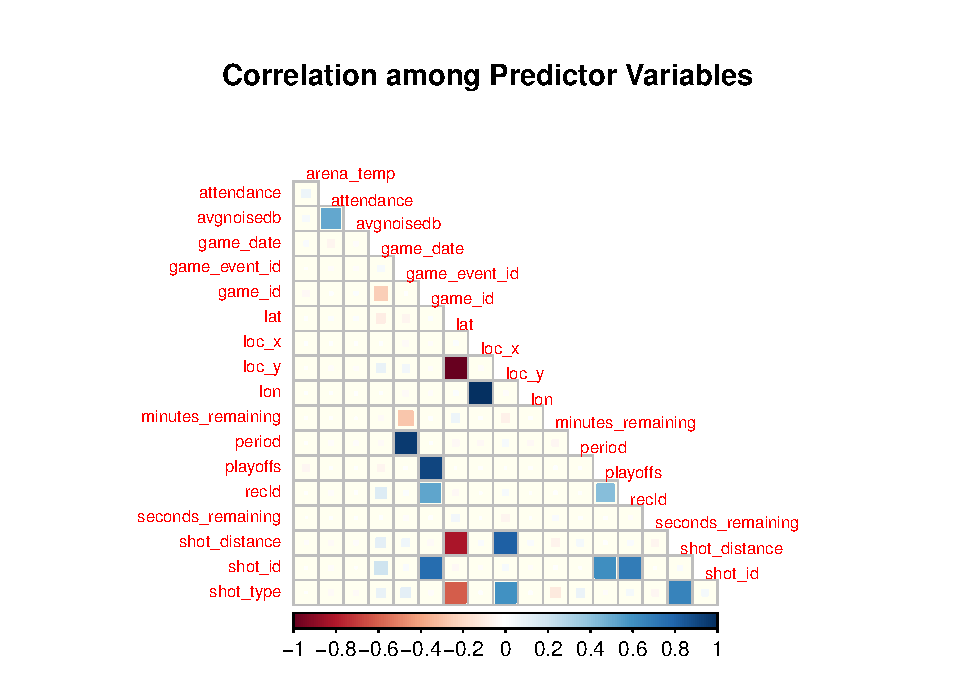
\includegraphics{Final_Project_Applied_files/figure-latex/Multicollinearity-1.pdf}

\hypertarget{post-correlation-plot-variable-elimination}{%
\subsection{\texorpdfstring{\textbf{Post-Correlation Plot Variable
Elimination}}{Post-Correlation Plot Variable Elimination}}\label{post-correlation-plot-variable-elimination}}

\hypertarget{following-our-correlation-plot-we-decided-to-eliminate-some-collinear-terms.-however-some-of-the-collinearity-is-useful-to-capture-the-instances-where-the-terms-are-unique.-for-example-combined_shot_type-factor-variable-is-collinear-with-shot_distance-quantitative-variable-but-it-also-accounts-for-the-method-kobe-may-use-to-make-a-shot.-for-example-distance-may-be-relatively-the-same-between-10-and-11-feet-but-the-factor-levels-used-to-derrive-their-short-or-far-indications-may-differ.-this-difference-could-be-whether-kobe-makes-a-potentially-more-accurate-heel-planted-shot-or-if-he-is-forced-to-lean-forward-and-take-a-riskier-shot-at-basket-the-difference-in-distance-may-only-be-one-foot-but-the-difference-in-technique-could-measure-significant-relative-to-the-odds-of-success.}{%
\subsubsection{\texorpdfstring{Following our correlation plot, we
decided to eliminate some collinear terms. However, some of the
collinearity is useful to capture the instances where the terms are
unique. For example, \texttt{combined\_shot\_type} (factor variable) is
collinear with \texttt{shot\_distance} (quantitative variable), but it
also accounts for the method Kobe may use to make a shot. For example,
distance may be relatively the same between 10 and 11 feet, but the
factor levels used to derrive their \texttt{short} or \texttt{far}
indications may differ. This difference could be whether Kobe makes a
potentially more accurate heel-planted shot or if he is forced to lean
forward and take a riskier shot at basket; the difference in distance
may only be one foot, but the difference in technique could measure
significant relative to the odds of
success.}{Following our correlation plot, we decided to eliminate some collinear terms. However, some of the collinearity is useful to capture the instances where the terms are unique. For example, combined\_shot\_type (factor variable) is collinear with shot\_distance (quantitative variable), but it also accounts for the method Kobe may use to make a shot. For example, distance may be relatively the same between 10 and 11 feet, but the factor levels used to derrive their short or far indications may differ. This difference could be whether Kobe makes a potentially more accurate heel-planted shot or if he is forced to lean forward and take a riskier shot at basket; the difference in distance may only be one foot, but the difference in technique could measure significant relative to the odds of success.}}\label{following-our-correlation-plot-we-decided-to-eliminate-some-collinear-terms.-however-some-of-the-collinearity-is-useful-to-capture-the-instances-where-the-terms-are-unique.-for-example-combined_shot_type-factor-variable-is-collinear-with-shot_distance-quantitative-variable-but-it-also-accounts-for-the-method-kobe-may-use-to-make-a-shot.-for-example-distance-may-be-relatively-the-same-between-10-and-11-feet-but-the-factor-levels-used-to-derrive-their-short-or-far-indications-may-differ.-this-difference-could-be-whether-kobe-makes-a-potentially-more-accurate-heel-planted-shot-or-if-he-is-forced-to-lean-forward-and-take-a-riskier-shot-at-basket-the-difference-in-distance-may-only-be-one-foot-but-the-difference-in-technique-could-measure-significant-relative-to-the-odds-of-success.}}

\hypertarget{addressing-multicollinearity-correlation-matrix-for-numerical-analysis}{%
\subsection{\texorpdfstring{\textbf{Addressing Multicollinearity:
Correlation Matrix for Numerical
Analysis}}{Addressing Multicollinearity: Correlation Matrix for Numerical Analysis}}\label{addressing-multicollinearity-correlation-matrix-for-numerical-analysis}}

\#\#\#Following the removal of the most obvious collinear terms visually
performing a correlation plot analysis, a correlation matrix for
analyzing the remaining results. Collinear quantitative data was
preliminarily removed following correlation plot analysis to desaturate
the model to an extent that allows more distinction among significance
measures for terms in the correlation matrix.

\begin{tabular}{l|l|l|l|r}
\hline
Row & Column & Correlation & p-value & NA\\
\hline
arena\_temp & arena\_temp & 0.510916827054281 & 0 & 0\\
\hline
attendance & arena\_temp & 0.510916827054281 & 0 & 0\\
\hline
game\_date & arena\_temp & 0.510916827054281 & 0 & 0\\
\hline
game\_event\_id & arena\_temp & 0.510916827054281 & 0 & 0\\
\hline
game\_id & arena\_temp & 0.510916827054281 & 0 & 0\\
\hline
loc\_x & arena\_temp & 0.510916827054281 & 0 & 0\\
\hline
loc\_y & arena\_temp & 0.510916827054281 & 0 & 0\\
\hline
minutes\_remaining & arena\_temp & 0.510916827054281 & 0 & 0\\
\hline
recId & arena\_temp & 0.510916827054281 & 0 & 0\\
\hline
seconds\_remaining & arena\_temp & 0.510916827054281 & 0 & 0\\
\hline
\end{tabular}

\hypertarget{after-the-first-round-of}{%
\section{After the first round of}\label{after-the-first-round-of}}

\hypertarget{quadratic-discriminant-analysis}{%
\section{\texorpdfstring{\textbf{Quadratic Discriminant
Analysis}}{Quadratic Discriminant Analysis}}\label{quadratic-discriminant-analysis}}

\hypertarget{as-requested-within-the-requirements-of-this-study-a-linear-discriminant-analysis-must-be-assessed-and-provided.-discriminant-analysis-is-an-operation-that-compares-a-categorical-response-variable-against-measures-of-quantitative-predictor-variables.-as-a-result-analysis-for-this-section-is-performed-on-the-numerical-predictors-which-include-recid-game_event_id-game_id-loc_x-loc_y-minutes_remaining-seconds_remaining-shot_distance-shot_made_flag-shot_type-game_date-shot_id-attendance-arena_temp-avgnoisedb-controlling-collinearity-by-eliminating-a-member-of-each-collinear-pair-prior-to-model-development.}{%
\subsubsection{\texorpdfstring{As requested within the requirements of
this study, a Linear Discriminant Analysis must be assessed and
provided. Discriminant analysis is an operation that compares a
categorical response variable against measures of quantitative predictor
variables. As a result, analysis for this section is performed on the
numerical predictors, which include \texttt{recId},
\texttt{game\_event\_id}, \texttt{game\_id}, \texttt{loc\_x},
\texttt{loc\_y}, \texttt{minutes\_remaining},
\texttt{seconds\_remaining}, \texttt{shot\_distance},
\texttt{shot\_made\_flag}, \texttt{shot\_type}, \texttt{game\_date},
\texttt{shot\_id}, \texttt{attendance}, \texttt{arena\_temp},
\texttt{avgnoisedb}, controlling collinearity by eliminating a member of
each collinear pair prior to model
development.}{As requested within the requirements of this study, a Linear Discriminant Analysis must be assessed and provided. Discriminant analysis is an operation that compares a categorical response variable against measures of quantitative predictor variables. As a result, analysis for this section is performed on the numerical predictors, which include recId, game\_event\_id, game\_id, loc\_x, loc\_y, minutes\_remaining, seconds\_remaining, shot\_distance, shot\_made\_flag, shot\_type, game\_date, shot\_id, attendance, arena\_temp, avgnoisedb, controlling collinearity by eliminating a member of each collinear pair prior to model development.}}\label{as-requested-within-the-requirements-of-this-study-a-linear-discriminant-analysis-must-be-assessed-and-provided.-discriminant-analysis-is-an-operation-that-compares-a-categorical-response-variable-against-measures-of-quantitative-predictor-variables.-as-a-result-analysis-for-this-section-is-performed-on-the-numerical-predictors-which-include-recid-game_event_id-game_id-loc_x-loc_y-minutes_remaining-seconds_remaining-shot_distance-shot_made_flag-shot_type-game_date-shot_id-attendance-arena_temp-avgnoisedb-controlling-collinearity-by-eliminating-a-member-of-each-collinear-pair-prior-to-model-development.}}

\hypertarget{section}{%
\subsubsection{}\label{section}}

\#\#\#Linear Discriminant Analysis requires a linear boundary between
the predictor variables, respective of the response. If the boundary
between predictors and response is not linear, Quadratic Discriminant
Analysis must be used. Wilks' Lambda distribution is used to assess the
nature of boundary linearity, which can be used for discriminant
analysis. However, because of the large dimensions of the data set
analyzed in this study, an approximation of Wilks' Lambda must be used.
Bartlett's Test is an approximation of Wilks' Lambda that can be used
for models with large dimensions by applying a measure against the
Chi-Square distribution. Provided is a test statistic and p-value.

\hypertarget{bartletts-test}{%
\subsubsection{\texorpdfstring{\textbf{Bartlett's
Test:}}{Bartlett's Test:}}\label{bartletts-test}}

\begin{longtable}[]{@{}lrrrl@{}}
\toprule
& Chi.Square.Statistic & Degrees.of.Freedom & Wilks..Lambda &
p.value\tabularnewline
\midrule
\endhead
Wilks' Lambda & 1036.917 & 14 & 0.9511137 & p \textless{}
0.0001\tabularnewline
\bottomrule
\end{longtable}

\hypertarget{bartletts-test-of-this-data-set-yielded-a-significant-p-value-where-p-0.0001-indicating-that-the-proportion-of-distribution-beyond-the-derrived-test-statistic-is-beyond-that-which-could-be-explained-by-chance.-therefore-we-must-reject-the-null-hypothesis-that-the-boundary-for-analysis-is-linear-the-boundary-is-non-linear.-thus-an-analysis-using-quadratic-discriminant-analysis-is-applied.}{%
\subsubsection{Bartlett's Test of this data set yielded a significant
p-value, where p \textless{} 0.0001, indicating that the proportion of
distribution beyond the derrived test statistic is beyond that which
could be explained by chance. Therefore, we must reject the null
hypothesis that the boundary for analysis is linear; the boundary is
non-linear. Thus, an analysis using Quadratic Discriminant Analysis is
applied.}\label{bartletts-test-of-this-data-set-yielded-a-significant-p-value-where-p-0.0001-indicating-that-the-proportion-of-distribution-beyond-the-derrived-test-statistic-is-beyond-that-which-could-be-explained-by-chance.-therefore-we-must-reject-the-null-hypothesis-that-the-boundary-for-analysis-is-linear-the-boundary-is-non-linear.-thus-an-analysis-using-quadratic-discriminant-analysis-is-applied.}}

\begin{verbatim}
##   mean.kobe.qda.posterior...1.. mean.kobe.qda.posterior...2..
## 1                      0.457789                      0.542211
\end{verbatim}

\begin{verbatim}
##   shot_made_flagg proportion
## 1               0   0.457789
## 2               1   0.542211
\end{verbatim}

\hypertarget{logistic-model-development-using-ordinary-least-squares}{%
\section{\texorpdfstring{\textbf{Logistic Model Development using
Ordinary Least
Squares}}{Logistic Model Development using Ordinary Least Squares}}\label{logistic-model-development-using-ordinary-least-squares}}

\hypertarget{a-preliminary-manual-veriable-elimination-process-was-performed-during-the-analysis-of-multicollinear-terms-in-preparation-for-model-development.-below-we-perform-logistic-regression-using-ordinary-least-squares-ols.-in-preparation-for-the-model-development-a-starting-model-and-a-finishing-model-must-be-developed-to-provide-the-scope-of-variable-selection.}{%
\subsubsection{A preliminary, manual veriable elimination process was
performed during the analysis of multicollinear terms in preparation for
model development. Below we perform logistic regression using Ordinary
Least Squares (OLS). In preparation for the model development, a
starting model and a finishing model must be developed to provide the
scope of variable
selection.}\label{a-preliminary-manual-veriable-elimination-process-was-performed-during-the-analysis-of-multicollinear-terms-in-preparation-for-model-development.-below-we-perform-logistic-regression-using-ordinary-least-squares-ols.-in-preparation-for-the-model-development-a-starting-model-and-a-finishing-model-must-be-developed-to-provide-the-scope-of-variable-selection.}}

\hypertarget{forward-selection}{%
\subsection{\texorpdfstring{\textbf{Forward
Selection}}{Forward Selection}}\label{forward-selection}}

\hypertarget{forward-selection-produced-a-model-that-produced-an-akaikes-information-criterion-score-of-27378.}{%
\subsubsection{Forward selection produced a model that produced an
Akaike's Information Criterion score of
27,378.}\label{forward-selection-produced-a-model-that-produced-an-akaikes-information-criterion-score-of-27378.}}

\hypertarget{section-1}{%
\subsubsection{}\label{section-1}}

\hypertarget{forward-selection-model}{%
\subsubsection{Forward Selection Model:}\label{forward-selection-model}}

\hypertarget{shot_made-flag-shot-distance-attendance-combined-shot-type-arena-temp-game-event-id-seconds-remaining-shot-type-game-date-minutes-remaining-loc-y-shot-id}{%
\subsubsection{\texorpdfstring{\(shot_made flag = shot distance + attendance + combined shot type + arena temp + game event id + seconds remaining + shot type + game date + minutes remaining + loc y + shot id\)}{shot\_made flag = shot distance + attendance + combined shot type + arena temp + game event id + seconds remaining + shot type + game date + minutes remaining + loc y + shot id}}\label{shot_made-flag-shot-distance-attendance-combined-shot-type-arena-temp-game-event-id-seconds-remaining-shot-type-game-date-minutes-remaining-loc-y-shot-id}}

\hypertarget{forward-selection---akaikes-information-criterion-for-logistic-regression}{%
\subsection{\texorpdfstring{\textbf{Forward Selection - Akaike's
Information Criterion for Logistic
Regression:}}{Forward Selection - Akaike's Information Criterion for Logistic Regression:}}\label{forward-selection---akaikes-information-criterion-for-logistic-regression}}

\begin{longtable}[]{@{}r@{}}
\toprule
Akaikes.Information.Criterion..Foreward.Selection\tabularnewline
\midrule
\endhead
26824.26\tabularnewline
\bottomrule
\end{longtable}

\hypertarget{backward-elimination}{%
\subsection{\texorpdfstring{\textbf{Backward
Elimination}}{Backward Elimination}}\label{backward-elimination}}

\hypertarget{backward-elimination-produced-a-model-that-produced-an-akaikes-information-criterion-score-of-27378.}{%
\subsubsection{Backward elimination produced a model that produced an
Akaike's Information Criterion score of
27,378.}\label{backward-elimination-produced-a-model-that-produced-an-akaikes-information-criterion-score-of-27378.}}

\hypertarget{section-2}{%
\subsubsection{}\label{section-2}}

\hypertarget{backward-elimination-model}{%
\subsubsection{Backward Elimination
Model:}\label{backward-elimination-model}}

\hypertarget{shot-made-flag-combined-shot-type-game-event-id-loc-y-minutes-remaining-seconds-remaining-shot-distance-shot-type-game-date-shot-id-attendance-arena-temp}{%
\subsubsection{\texorpdfstring{\(shot made flag = combined shot type + game event id + loc y + minutes remaining + seconds remaining + shot distance + shot type + game date + shot id + attendance + arena temp\)}{shot made flag = combined shot type + game event id + loc y + minutes remaining + seconds remaining + shot distance + shot type + game date + shot id + attendance + arena temp}}\label{shot-made-flag-combined-shot-type-game-event-id-loc-y-minutes-remaining-seconds-remaining-shot-distance-shot-type-game-date-shot-id-attendance-arena-temp}}

\hypertarget{backward-elmination---akaikes-information-criterion-for-logistic-regression}{%
\subsection{\texorpdfstring{\textbf{Backward Elmination - Akaike's
Information Criterion for Logistic
Regression:}}{Backward Elmination - Akaike's Information Criterion for Logistic Regression:}}\label{backward-elmination---akaikes-information-criterion-for-logistic-regression}}

\begin{longtable}[]{@{}r@{}}
\toprule
Akaikes.Information.Criterion..Backward.Elimination\tabularnewline
\midrule
\endhead
26824.26\tabularnewline
\bottomrule
\end{longtable}

\hypertarget{stepwise-regression}{%
\subsection{\texorpdfstring{\textbf{Stepwise
Regression}}{Stepwise Regression}}\label{stepwise-regression}}

\hypertarget{stepwise-regression-produced-a-model-that-produced-an-akaikes-information-criterion-score-of-27378.}{%
\subsubsection{Stepwise Regression produced a model that produced an
Akaike's Information Criterion score of
27,378.}\label{stepwise-regression-produced-a-model-that-produced-an-akaikes-information-criterion-score-of-27378.}}

\hypertarget{section-3}{%
\subsubsection{}\label{section-3}}

\hypertarget{stepwise-regression-model}{%
\subsubsection{Stepwise Regression
Model:}\label{stepwise-regression-model}}

\hypertarget{shot-made-flag-combined-shot-type-game-event-id-loc-y-minutes-remaining-seconds-remaining-shot-distance-shot-type-game-date-shot-id-attendance-arena-temp-1}{%
\subsubsection{\texorpdfstring{\(shot made flag = combined shot type + game event id + loc y + minutes remaining + seconds remaining + shot distance + shot type + game date + shot id + attendance + arena temp\)}{shot made flag = combined shot type + game event id + loc y + minutes remaining + seconds remaining + shot distance + shot type + game date + shot id + attendance + arena temp}}\label{shot-made-flag-combined-shot-type-game-event-id-loc-y-minutes-remaining-seconds-remaining-shot-distance-shot-type-game-date-shot-id-attendance-arena-temp-1}}

\hypertarget{stepwise-regression---akaikes-information-criterion-for-logistic-regression}{%
\subsection{\texorpdfstring{\textbf{Stepwise Regression - Akaike's
Information Criterion for Logistic
Regression:}}{Stepwise Regression - Akaike's Information Criterion for Logistic Regression:}}\label{stepwise-regression---akaikes-information-criterion-for-logistic-regression}}

\begin{longtable}[]{@{}r@{}}
\toprule
Akaikes.Information.Criterion..Stepwise.Regression\tabularnewline
\midrule
\endhead
26824.26\tabularnewline
\bottomrule
\end{longtable}


\end{document}
